\documentclass{article}

% if you need to pass options to natbib, use, e.g.:
%     \PassOptionsToPackage{numbers, compress}{natbib}
% before loading neurips_2020

% ready for submission
% \usepackage{neurips_2020}

% to compile a preprint version, e.g., for submission to arXiv, add add the
% [preprint] option:
%     \usepackage[preprint]{neurips_2020}

% to compile a camera-ready version, add the [final] option, e.g.:
%     \usepackage[final]{neurips_2020}

% to avoid loading the natbib package, add option nonatbib:
     \usepackage[nonatbib]{neurips_2020}

\usepackage[utf8]{inputenc} % allow utf-8 input
\usepackage[T1]{fontenc}    % use 8-bit T1 fonts
\usepackage{hyperref}       % hyperlinks
\usepackage{url}            % simple URL typesetting
\usepackage{booktabs}       % professional-quality tables
\usepackage{amsfonts}       % blackboard math symbols
\usepackage{nicefrac}       % compact symbols for 1/2, etc.
\usepackage{microtype}      % microtypography
\usepackage[english]{babel}
\usepackage[utf8]{inputenc}
\usepackage{listings}
\usepackage{color}
\usepackage{algorithm}
\usepackage{algorithmic}
\usepackage{todonotes}
\usepackage{siunitx}
\usepackage{authblk}
\usepackage{subcaption}
\usepackage{bbm}
\usepackage{amsmath}

\graphicspath{ {.} }
\include{Commands}
\newtheorem{theorem}{Theorem}

\definecolor{dkgreen}{rgb}{0,0.6,0}
\definecolor{gray}{rgb}{0.5,0.5,0.5}
\definecolor{mauve}{rgb}{0.58,0,0.82}

\lstset{frame=tb,
	language=C,
	aboveskip=3mm,
	belowskip=3mm,
	showstringspaces=false,
	columns=flexible,
	basicstyle={\small\ttfamily},
	numbers=none,
	numberstyle=\tiny\color{gray},
	keywordstyle=\color{blue},
	commentstyle=\color{dkgreen},
	stringstyle=\color{mauve},
	breaklines=true,
	breakatwhitespace=true,
	tabsize=3
}

\title{BitTensor: A Peer-to-Peer Intelligence Benchmark}

% The \author macro works with any number of authors. There are two commands
% used to separate the names and addresses of multiple authors: \And and \AND.
%
% Using \And between authors leaves it to LaTeX to determine where to break the
% lines. Using \AND forces a line break at that point. So, if LaTeX puts 3 of 4
% authors names on the first line, and the last on the second line, try using
% \AND instead of \And before the third author name.
  % examples of more authors
  % \And
  % Coauthor \\
  % Affiliation \\
  % Address \\
  % \texttt{email} \\
  % \AND
  % Coauthor \\
  % Affiliation \\
  % Address \\
  % \texttt{email} \\
  % \And
  % Coauthor \\
  % Affiliation \\
  % Address \\
  % \texttt{email} \\
  % \And
  % Coauthor \\
  % Affiliation \\
  % Address \\
  % \texttt{email} \\


\begin{document}

\maketitle

\begin{abstract}
The dominant tools used to guide machine intelligence are typically benchmarks which rank systems on a set of predefined tasks. However, task performance is a narrowly defined, low-resolution, and non-collaborative measure making it an inefficient guide for machine intelligence. Instead, we propose a benchmark that measures \textit{knowledge production} from within a network of intelligence systems. In this paper we describe how this benchmark is constructed and how it is negotiated by computers that share what they learn peer-to-peer (P2P) across the internet. Since this internet based negotiation introduces game-theoretic considerations, we design methods to improve the benchmark's accuracy when peers remain self-interested and trustless. We then test our design by empirically showing that the negotiation closely matches the desired ranking at the system's competitive equilibrium. 

%The result is a benchmark that is inherently collaborative, efficient, and decentralized.
\end{abstract}

Increasingly, state-of-the-art machine learning systems focus on the production of \textit{machine knowledge}: non-task specific understanding of inputs which can be later tuned to a wide variety of problems \cite{devlin2018bert}. This shift is a consequence of the fact that a focus on tasks during training produces narrow specialists rather than resilient generalists \cite{radford2019language}. However, while becoming the dominant technique for training individual models, the field still opts for task based objectives as the method of reward at the highest level of its evolution \cite{wang2018glue}. We suggest this introduces wide-scale inefficiencies into the advancement of machine intelligence for the following reasons:

\begin{enumerate}
	\item Guiding machine intelligence with performance on a  small number of tasks converges the field towards narrow specialists \cite{chollet2019measure}. Unfortunately, simply expanding the set tasks to cover the general problem would require a large number of expensive supervised (dataset, task) pairs \cite{radford2019language}. This intractability suggests task-based feedback mechanisms cannot alone guide machine intelligence towards a high level of generalism. In contrast, task agnostic knowledge can be extracted using unsupervised techniques and measured against a near infinite amount of cheap unlabelled data \cite{devlin2018bert}. The fact that this knowledge can then be used to solve many tasks \cite{radford2019language} suggests that it may also provide a much broader definition of intelligence against which to benchmark. 
	
	\item Canonical task based intelligence benchmarks produce a small number of scores (i.e accuracy on 8 tasks \cite{wang2019superglue}) to measure the performance of the models which they evaluate. While conveniently human interpretable, the scores are low resolution substitutes for the information produced by the models. The language model BERT, for instance, produces a 1024 dimensional continuous distribution over sentences; an ensemble could directly learn from this distribution and rank it in combination with others \cite{shazeer2017outrageously}. By lacking this resolution benchmarks fail to reward niche machine intelligence systems and the knowledge they have uncovered.
	
	\item Task based benchmarks do not measure the  Task based benchmarks produce a winner-take-all competition which prunes all but the best. The result is a world-wide challenge where only those with the means and the resources to train the largest models may contribute to the state-of-the-art.
\end{enumerate}


A benchmark that directly measures machine knowledge production would be very beneficial  \footnote{“The iron rule of nature is: you get what you reward for. If you want ants to come, you put sugar on the floor.” - Charlie Munger}. By analogy, similar to rewarding domain specialists or generalists in human cultures -- not against their ability to solve tasks -- but their ability to improve overall understanding. Our proposal is a framework in which models directly share knowledge that they have learned with each other. Their peers select that knowledge for its ability to improve their own understanding. Crucially, each model's performance is measured by its ability to improve collective understanding of inputs rather than against any specific task. {\color{red} This re-framing of the measurement technique allows the system to reward models for improving small regions of the general problem. Inherently, the benchmark introduces knowledge sharing, while the demand for performance guides a de-facto ``market for intelligence".   }

Practically, we design the benchmark to run in a continuous and asynchronous fashion, peer-to-peer (P2P) across the Internet. Since this introduces trustless computation \footnote{ In decentralized systems, trust is shifted from the individuals to the network itself, "trustless" usually means "minimal trust is required" with respect to the protocol} we dedicate a part of this paper to explaining how the system remains fair when little assurance can be given about the computers that compose it. In summary, the contributions of this paper are thus four-fold:
\begin{enumerate}
	\item We introduce a P2P based intelligence framework.
	\item We introduce an ``intelligence market" that rewards models that improve representational knowledge within the network.
	\item We show how models can share knowledge to increase each other's performance, which removes the need for others to re-learn that knowledge. 
	\item We show how a self-interested desire to minimize a loss function can be used to guide the network towards a fair ranking.
\end{enumerate}

The rest of this paper is organized as follows: Section~\ref{methodology} presents the intelligence benchmark and ranking mechanism that models use to evaluate each other. Section~\ref{analysis} proposes a method to detect and respond to the scenario where participants are not honestly reporting the significance of their peers. Section ~\ref{experiments} highlights the experiments performed to verify the function of this framework. Finally, Section~\ref{conclusion} presents a summary and future works on this system.

\section{Methodology}
\label{methodology}

\subsection{Benchmark}

The network is composed by $n$ unique parameterized functions $F = {f_0, ...,  f_j, ...f_n}$ where each function is producing an output tensor $f_i(F(x))$, a ``representation" from an input tensor $F(x) = [f_0{(x)} ... f_n{(x)}]$ gathered by querying its neighbors. Each function is training asynchronously over a dataset $D_i=[X,Y]$ such that, given an error function $\mathcal{Q}_i$, its expectation over that data $E_{Di}$ defines a loss $\mathcal{L}_i = E_{Di}[\mathcal{Q}_i( \ y, \ f_i(F(x)) \ )]$. We assume these losses are measured on the same scale and thus our benchmark $\mathcal{B}$ can be defined by their sum:

\begin{equation}
\mathcal{B} = \ \sum_{i}^{n} \mathcal{L}_i 
\end{equation}

\begin{figure}[H]
	\centering
	\hspace*{-2cm}
	\begin{center}
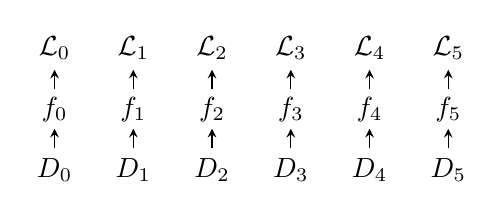
\begin{tikzpicture}
\begin{scope}[scale=0.5]
    
    
    \node (a) at (0,0) [rectangle, rounded corners] {$f_0$};
    \node (b) at (2,0) [rectangle, rounded corners] {$f_1$};
    \node (c) at (4,0) [rectangle, rounded corners] {$f_2$};
    \node (d) at (6,0) [rectangle, rounded corners] {$f_3$};
    \node (e) at (8,0) [rectangle, rounded corners] {$f_4$};
    \node (f) at (10,0) [rectangle, rounded corners] {$f_5$};
    
    \draw[-stealth] (0,0.5) -- (0, 1) node[above] {$\mathcal{L}_0$};
    \draw[-stealth] (2,0.5) -- (2, 1) node[above] {$\mathcal{L}_1$};
    \draw[-stealth] (4,0.5) -- (4, 1) node[above] {$\mathcal{L}_2$};
    \draw[-stealth] (6,0.5) -- (6, 1) node[above] {$\mathcal{L}_3$};
    \draw[-stealth] (8,0.5) -- (8, 1) node[above] {$\mathcal{L}_4$};
    \draw[-stealth] (10,0.5) -- (10, 1) node[above] {$\mathcal{L}_5$};

    
    \draw[-stealth] (0, -1) node[below] {$D_0$} -- (0, -0.5);
    \draw[-stealth] (2, -1) node[below] {$D_1$} -- (2, -0.5);
    \draw[-stealth] (4, -1) node[below] {$D_2$} -- (4, -0.5);
    \draw[-stealth] (6, -1) node[below] {$D_3$} -- (6, -0.5);
    \draw[-stealth] (8, -1) node[below] {$D_4$} -- (8, -0.5);
    \draw[-stealth] (10, -1) node[below] {$D_5$} -- (10, -0.5);
    
\end{scope}
\end{tikzpicture}
\end{center}

	%    \label{fig:progdense_diagram}
	\caption{$n=6$ parameterized functions with losses $\mathcal{L}_i$ and datasets $D_i$.}
\end{figure}{}

Each parameterized function is represented here in its most abstract sense\cite{hinton2015distilling} and need only accept the same input type $x$ and produce the same output dimension to fit within the network. {\color{blue} For instance, unicode encoded string $x = "hello"$ and its semantic representation as a $64x49$ word embedding.} This widened scope ensures participants can be multi-task \cite{kaiser2017model}, use completely distinct computing substrates \cite{alex2014cortical} or train on unique datasets. \cite{lample2019crosslingual}. 

\subsection{Ideal Ranking}

Our goal in this work is to produce a ranking $R = [R_i]$ over these functions where the score $R_i \in R$ represents participant $i$'s information-theoretic significance to the benchmark $\mathcal{B}$. Following Le Cun and others \cite{lecun1989optimalbraindamage,yu2017nisp}, it is reasonable to analytically define this significance by equating it with the cost of removing each component from the network:

\begin{equation}
\label{eq:r}
R_i \approx \ \ \frac{1}{n} \sum_{j}^{n} \sum_{x \in D_j} \Delta F^T(x)_i * H(\mathcal{Q}_j(x)) * \Delta F(x)_i 
\end{equation}

\[ \Delta F (x)_i = [0, ... 0, -f_i(x), 0, ... 0] \]

Where the above is derived using a Taylor series (Appendix 6.1) and $\Delta F (x)_i$ is the {\color{blue} perturbation of the $i^{th}$ node's inputs as a function of it's choice of weights when removing function $f_i$ at the point $x$}. Note, the linear and higher order terms of the Taylor series have been removed following \cite{yu2017nisp} and the remaining term $H(\mathcal{Q}_i)$ is the hessian of our error function. When the error function $\mathcal{Q}$ is the twice-differentiable cross-entropy, then $H(\mathcal{Q}_i)$ is the Fisher information matrix, and $R_i \in R$ is measured as relative entropy: reflects each participants informational significance to the network as a whole.

\subsection{Inter Ranking}
\label{sec:inter-ranking}
It is not possible to compute the ranking score above without access to the parameters of each function in the network. Instead, we use a set of inter-model weights $W = [w_{i_j}]$ where each $w_{i,j}$ is the score attributed to $f_j$ from $f_i$ combined into an $n \times n$ square matrix.

\begin{equation}
\label{eq:w}
w_{ij} = \ \ \sum_{x \in D_i} \Delta F^T(x)_j * H(\mathcal{Q}_i(x)) * \Delta F(x)_j
\end{equation}

\begin{figure}[H]
	\centering
	\hspace*{-2cm}
	\begin{center}

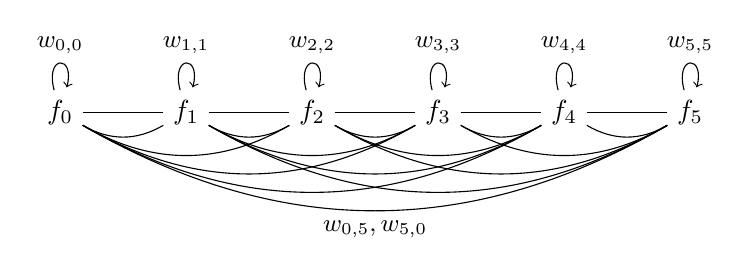
\begin{tikzpicture}


\begin{scope}[scale=0.8]

    \node (a) at (0,0) [rectangle] {$f_0$};
    \node (b) at (2,0) [rectangle] {$f_1$};
    \node (c) at (4,0) [rectangle] {$f_2$};
    \node (d) at (6,0) [rectangle] {$f_3$};
    \node (e) at (8,0) [rectangle] {$f_4$};
    \node (f) at (10,0) [rectangle] {$f_5$};
    
  
    \path[every node/.style={font=\sffamily\small}]
        (a) edge node [right] {} (b)
        (b) edge node [right] {} (c)
        (c) edge node [right] {} (d)
        (c) edge node [right] {} (d)
        (d) edge node [right] {} (e)
        (e) edge node [right] {} (f)


        (a) edge [loop above]  node[above]  {$w_{0,0}$} (a)
        (b) edge [loop above]  node[above]  {$w_{1,1}$} (b)
        (c) edge [loop above]  node[above]  {$w_{2,2}$} (c)
        (d) edge [loop above]  node[above]  {$w_{3,3}$} (d)
        (e) edge [loop above]  node[above]  {$w_{4,4}$}  (e)
        (f) edge [loop above]  node[above]  {$w_{5,5}$}  (f)

        (a) edge [bend right]  (b)
        (a) edge [bend right]  (c)
        (a) edge [bend right]  (d)
        (a) edge [bend right]  (e)
        (a) edge [bend right]  node[below]  {$w_{0,5}, w_{5,0}$}(f)
        (b) edge [bend right]  (c)
        (b) edge [bend right]  (d)
        (b) edge [bend right]  (e)
        (b) edge [bend right]  (f)
        (c) edge [bend right]  (d)
        (c) edge [bend right]  (e)
        (c) edge [bend right]  (f)
        (d) edge [bend right]  (e)
        (d) edge [bend right]  (f)
        (e) edge [bend right]  (f);
    
\end{scope}


\end{tikzpicture}
\end{center}

	%    \label{fig:progdense_diagram}
	\caption{Inter-model contribution weights: $w_{i,j}$ the score attributed to $f_j$ from $f_i$}
\end{figure}{}

%{\color{blue} -- e.g. by using a heuristic to propagate the weights from the final layer of $f_i$ through to the first layer of $f_j$ --}  

The weights can be computed on the fly either approximately \cite{yu2017nisp} or by using the full hessian of the error. We store them on a distributed ledger and allow participants to update them by making changes of bounded size: $W^{t+1}= W^t + \lambda \Delta W$, where $||W_i||_2 < \epsilon$ at block step $t$. We also enforce that the scores in each row sum to 1, $||w||_1 = 1$. {\color{blue} The reasoning for this enforcement is to ensure stake fairness between early movers and newcomers with innovations that enable them to perform better overall.}

The equivalent ranking $R$ in Equation ~(\ref{eq:r}) can then be computed by normalizing column sum of the weight matrix:

\begin{equation}
\label{eq:equiv_ranking}
R = \frac{1}{n} W^T * \mathbbm{1}
\end{equation}

The problem is that without system-wide access to the model parameters, the computation of $w_{ij}$ in Equation (\ref{eq:w}) is intractable, {\color{blue} as it would require collecting great amounts of information from potentially billions of neurons}. It is reasonable to assume participants will select weights which artificially increase their own rank rather than others in the network. Moreover, since the network remains open, participants may choose to create many spuriously neighbours and rank themselves higher. The remainder of this paper describes our proposal for resolving these issues.

\subsection{Stake}
\label{sec:stake}
The proposed solution begins by introducing a finite resource $ S=[s_i]$, a component's 'stake' in the system, and an inflation mechanism $\tau$ which translates the ranking vector $R$ into additional stake as incentive. 

\begin{equation}
\label{eq:r_stake}
R = \frac{1}{n} W^T \circ S * \mathbbm{1}
\end{equation}

\begin{equation}
S^{t+1} = S^t + \tau * \frac{R}{||R||_2} 
\end{equation}

The $\circ$ represents Hadamard product between the $n \times n$ matrix $W$ and the $n \times n$ matrix containing $S$ in each column, and $t$ is the time-step referred to in Section~\ref{sec:inter-ranking} (measured in distinct blocks on the distributed ledger). By design Equation (\ref{eq:r_stake}) increases the importance of those with stake, $s_0 * w_{ij}$. This serves two purposes: 

\begin{enumerate}
	\item New computers can spuriously create new nodes, however this won't game the ranking because the amount of stake they hold is finite.
	\item The resource provides mechanism power.
\end{enumerate}

By providing it to nodes with large rank, this ensures that those with weight must have worked to attain it, or indirectly subsidized those who have done so already. A single staked token would be enough to bootstrap the process. \footnote{The propagation of a resource mocks the flow of the brain-derived neurotrophic factor (BDNF). \cite{Bathina1989neurotrophin}} 

\begin{algorithm}
	\caption{Inflation mechanism}
	\begin{algorithmic} 
		
		\REQUIRE $S = \ [n \times 1] \ \textrm{Stake Vector}$
		\REQUIRE $W = \ [n \times n] \ \textrm{Weight Matrix}$
		\REQUIRE $\tau > 0 \ \textrm{inflation rate}$
		\WHILE{$\text{TRUE}$}
		\STATE $W = W + \lambda \Delta W$
		\STATE $R = \frac{1}{n} W^T \circ S * \mathbbm{1}$
		\STATE $S = S + \tau * \frac{R}{||R||_2}  $
		\ENDWHILE
	\end{algorithmic}
\end{algorithm}

\subsection{Competitive weights}
\label{sec:competitive_weights}
While stake provides some protection against malicious actors, it does not ensure weights are set accurately. Our solution begins by introducing competition for connectivity within the network. Nodes that underweight are punished by having inputs from the network masked to zero~(\ref{eq:7}), {\color{blue} which in turn would punish the loss function}. To frame this market we borrow the continuous differential activation function $\sigma$ with range $(0,1)$. Under a choice of weights $W_i$ the inputs to component $i$ are:

\begin{equation}
\label{eq:7}
F_W(x) =  [f_0(x) * \sigma(s_i * w_{i,0} - \mu_0),  ... , f_n(x) * \sigma(s_i * w_{i,n} - \mu_n)]
\end{equation}

\begin{equation}
\sigma =  \frac{1}{ 1 + e^{-\frac{x}{T}} }
\end{equation}

Here, the shift term $\mu_j$ is the average of the weights in each column $\mu_j = (\frac{1}{n}) \sum_{i}^{n}{s_i * w_{i,j}}$, and the activation function is the temperature scaled sigmoid. Because the allocation mechanism is standard across the network it is possible for each participants to compute both $\frac{\partial \mathcal{L}_i}{\partial W_i}$ and $\frac{\partial R_i}{\partial W_i}$. Computers may augment their usual training framework, for instance, Tensorflow, with the allocation mechanism shown here. 

\subsection{Running the network}

The steps to run a network participant are:
\begin{enumerate}
	
	\item Participant defines its dataset $D_i$, loss $\mathcal{L}_i$ and parameterized function $f_i$
	\item  At each training iteration the participant broadcasts batches of examples from $D_i$ to its peers $[\textit{batch\_size}, x]$
	\item Responses $F(x)$ from the network produce a loss-gradient $\frac{\partial \mathcal{L}}{\partial F}$ which back-propagates through $f_i$ and out to the network.
	\item  During 2 and 3 the participant competitively selects the weights for their row $w_{ij} \in W$.
	\item  Participants submit changes to the weights $\Delta W_i$ which, in-turn changes the ranking and induces inflation $\tau * R$.
	\item  {\color{blue} After steps 1-5 have been performed multiple times}, participants disconnect and verify the model in a normal manner.
\end{enumerate}

Peers only communicate with computers that hold stake as a consequence of section~\ref{sec:competitive_weights}. Those that fail to produce value will be pruned naturally as participants learn to differentiate signal from noise.

\subsection{Conditional computation}

As the network grows, outward bandwidth will become the major bottleneck. Components learn to trim outward bandwidth by employing a Sparsely-Gated Mixture-of-Experts (SGMoE) \cite{shazeer2017outrageously} layer at the input. The gating layer determines a sparse combination of children to query for each example and then re-joins them using the the gating weights $g_j(x)$. The combined gated inputs are fed as input to the local function: 

\begin{equation}
f_i = f_i(G(x)) \ \ \ \  \textrm{ }
\end{equation}

\begin{equation}
\label{eq:gating_ensemble}
G(x) = [ ..., g_j(x) * f_j(x), ...]
\end{equation}


The layer cuts outward bandwidth, querying only a small subset of peers for each example. The gating function is trainable w.r.t to the loss and its weights act as a proxy for importance $w_{ij} \in W$. This method has been shown to drastically increase the potential for outward bandwidth in datacenter training,\cite{shazeer2017outrageously} and has been investigated in a peer-to-peer (P2P) setting as well \cite{Riabinin2020learningathome}


\subsection{Extracting knowledge}

Inter-node dependence in the network is broken using distillation\cite{hinton2015distilling}, a compression and knowledge technique in which a smaller model -- the student - mimics the behaviour of an ensemble. We employ this technique over the gating ensemble described in Equation (\ref{eq:gating_ensemble}) where the student model learns to minimize the cross-entropy (shown below as KL) between the logits produced by the gating network and its predicted distribution. \cite{Sanh2019DistilBERT}

\begin{equation}
\textrm{distillation loss} = \text{KL}_D(\text{dist}(x), G(x)) 
\end{equation}

We use the distilled model as proxy to cut recursive calling between each components rather than query farther into the network. If models go offline, their peers can use their distilled versions in-place. Private data can be validated over the distilled models instead of querying the network. Eventually, components can fully disconnect from the network using the distilled inputs to validate and inference the models offline.

\begin{figure}[H]
	\centering
	\hspace*{0cm}
	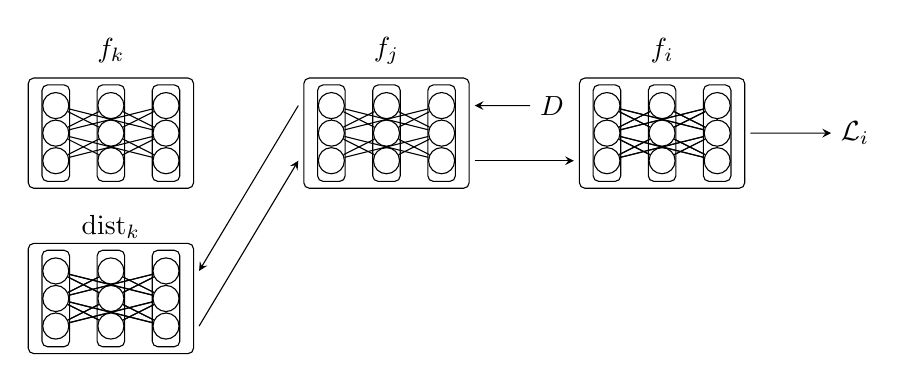
\begin{tikzpicture}


\begin{scope}[scale=0.7]

    \node[] at (1,2) {$f_j$};
    \node[] at (-4,2) {$f_k$};
    \node[] at (6,2) {$f_i$};
    
    \node[] at (-4,-1.2) {$\text{dist}_k$};

    

    %\draw[-stealth] (-7,3) node[below] {$\mathbf{M_1}$} -- (-5.5, 0.5);
    %\draw[-stealth] (-2.5, 0.5) -- (-1.5, 1.75) node[above] {$\mathcal{L}_k$};
    %\draw[-stealth] (2.5, 0.5) -- (3.5, 1.75) node[above] {$\mathcal{L}_j$};
    
    \node[] (m) at (4, 1) {$D$};
    \node[] (l) at (9.5, 0.5) {$\mathcal{L}_i$};
    
    \draw[-stealth] (m) -- (2.6, 1);
    \draw[-stealth] (7.6, 0.5) -- (l);

    
   % \draw[-stealth] (7.5, 0.5) -- (8.5, 1.75) node[above] {$\mathcal{L}_i$};
    
    \draw[-stealth] (2.6, 0) -- (4.4, 0);
    \draw[-stealth] (-0.6, 1) -- (-2.4, -2.0);
    \draw[-stealth] (-2.4, -3) -- (-0.6, 0);
    

    \foreach \x in {0,...,2}
        {
        \foreach \y in {0,...,2} 
            {
            \node[circle, draw, scale=1] (\x\y) at (\x, \y * 0.5) {};
            }
        \draw[rounded corners=2] (\x - 0.25, 1.375) rectangle ++(0.5, -1.75);
        }
    \draw[rounded corners=2] (-0.5, -0.5) rectangle ++(3, 2);
    
    
    \foreach \x in {0,...,2}
        {
        \foreach \y in {1,2}
            {
            \pgfmathsetmacro\yi{int(\y - 1)}
            \draw (\x\yi)edge(0\y);
            \draw (\x\yi)edge(1\y);
            \draw (\x\yi)edge(2\y);
            }
        }
        
     \foreach \x in {0,...,2}
        {
        \foreach \y in {0,...,2} 
            {
            \node[circle, draw, scale=1] (\x\y) at (\x - 5, \y * 0.5) {};
            }
        \draw[rounded corners=2] (\x - 0.25 - 5, 1.375) rectangle ++(0.5, -1.75);
        }
    \draw[rounded corners=2] (-0.5 - 5, -0.5) rectangle ++(3, 2);

    
    \foreach \x in {0,...,2}
        {
        \foreach \y in {1,2}
            {
            \pgfmathsetmacro\yi{int(\y - 1)}
            \draw (\x\yi)edge(0\y);
            \draw (\x\yi)edge(1\y);
            \draw (\x\yi)edge(2\y);
            }
        }
        
    \foreach \x in {0,...,2}
        {
        \foreach \y in {0,...,2} 
            {
            \node[circle, draw, scale=1] (\x\y) at (\x + 5, \y * 0.5) {};
            }
        \draw[rounded corners=2] (\x - 0.25 + 5, 1.375) rectangle ++(0.5, -1.75);
        }
    \draw[rounded corners=2] (-0.5 + 5, -0.5) rectangle ++(3, 2);

    
    \foreach \x in {0,...,2}
        {
        \foreach \y in {1,2}
            {
            \pgfmathsetmacro\yi{int(\y - 1)}
            \draw (\x\yi)edge(0\y);
            \draw (\x\yi)edge(1\y);
            \draw (\x\yi)edge(2\y);
            }
        }
        
        
    %  \foreach \x in {0,...,2}
    %     {
    %     \foreach \y in {0,...,2} 
    %         {
    %         \node[circle, draw, scale=1] (\x\y) at (\x, \y * 0.5 - 4) {};
    %         }
    %     \draw[rounded corners=2] (\x - 0.25, 1.375 - 4) rectangle ++(0.5, -1.75);
    %     }
    % \draw[rounded corners=2] (-0.5, -0.5 - 4) rectangle ++(3, 2);

    
    \foreach \x in {0,...,2}
        {
        \foreach \y in {1,2}
            {
            \pgfmathsetmacro\yi{int(\y - 1)}
            \draw (\x\yi)edge(0\y);
            \draw (\x\yi)edge(1\y);
            \draw (\x\yi)edge(2\y);
            }
        }
        
     \foreach \x in {0,...,2}
        {
        \foreach \y in {0,...,2} 
            {
            \node[circle, draw, scale=1] (\x\y) at (\x - 5, \y * 0.5 - 3) {};
            }
        \draw[rounded corners=2] (\x - 0.25 - 5, 1.375 - 3) rectangle ++(0.5, -1.75);
        }
    \draw[rounded corners=2] (-0.5 - 5, -0.5- 3) rectangle ++(3, 2);

    
    \foreach \x in {0,...,2}
        {
        \foreach \y in {1,2}
            {
            \pgfmathsetmacro\yi{int(\y - 1)}
            \draw (\x\yi)edge(0\y);
            \draw (\x\yi)edge(1\y);
            \draw (\x\yi)edge(2\y);
            }
        }
        
    %  \foreach \x in {0,...,2}
    %     {
    %     \foreach \y in {0,...,2} 
    %         {
    %         \node[circle, draw, scale=1] (\x\y) at (\x + 5, \y * 0.5 - 4) {};
    %         }
    %     \draw[rounded corners=2] (\x - 0.25 + 5, 1.375 - 4) rectangle ++(0.5, -1.75);
    %     }
    % \draw[rounded corners=2] (-0.5 + 5, -0.5- 4) rectangle ++(3, 2);

    
    \foreach \x in {0,...,2}
        {
        \foreach \y in {1,2}
            {
            \pgfmathsetmacro\yi{int(\y - 1)}
            \draw (\x\yi)edge(0\y);
            \draw (\x\yi)edge(1\y);
            \draw (\x\yi)edge(2\y);
            }
        }
        
 
    
    
    % \foreach \y in {0,...,2}
    %     {
    %     \foreach \x in {0,...,2} 
    %         {
    %         \pgfmathsetmacro\xi{(6 + \x*0.5)}
    %         \node[circle, draw] (\x\y) at (\xi,\y) {};
    %         }
    %     \draw[rounded corners=2] (6 + -0.375,\y+0.25) rectangle ++(1.75,-0.5);
    %     }
    % \draw[rounded corners=2] (6 + -0.5, -0.4) rectangle ++(2, 2.8);

    
    % \foreach \x in {0,...,2}
    %     {
    %     \foreach \y in {1,2}
    %         {
    %         \pgfmathsetmacro\yi{int(\y - 1)}
    %         \draw (\x\yi)edge(0\y);
    %         \draw (\x\yi)edge(1\y);
    %         \draw (\x\yi)edge(2\y);
    %         }
    %     }
        
    % \draw[-stealth] (6 + 0.5,-1) node[below] {$\mathbf{M_1}$} -- (6 + 0.5,-0.5);
    % \draw[-stealth] (6 + 0.5,2.5) -- (6 + 0.5,3) node[above] {$\mathcal{L}_1$};
    
    
    % \foreach \y in {0,...,2}
    %     {
    %     \foreach \x in {0,...,2} 
    %         {
    %         \pgfmathsetmacro\xi{(6 + \x*0.5)}
    %         \node[circle, draw] (\x\y) at (\xi,-6 +  \y) {};
    %         }
    %     \draw[rounded corners=2] (6 + -0.375, -6 + \y+0.25) rectangle ++(1.75,-0.5);
    %     }
    % \draw[rounded corners=2] (6 + -0.5, -6 + -0.4) rectangle ++(2, 2.8);

    
    % \foreach \x in {0,...,2}
    %     {
    %     \foreach \y in {1,2}
    %         {
    %         \pgfmathsetmacro\yi{int(\y - 1)}
    %         \draw (\x\yi)edge(0\y);
    %         \draw (\x\yi)edge(1\y);
    %         \draw (\x\yi)edge(2\y);
    %         }
    %     }
        
    % \draw[-stealth] (6 + 0.5, -6 + -1) node[below] {$\mathbf{M_2}$} -- (6 + 0.5, -6 +  -0.5);
    % \draw[-stealth] (6 + 0.5, -6 + 2.5) -- (6 + 0.5, -6 + 3) node[above] {$\mathcal{L}_2$};
    
    
    %  \foreach \y in {0,...,2}
    %     {
    %     \foreach \x in {0,...,2} 
    %         {
    %         \pgfmathsetmacro\xi{(12 + \x*0.5)}
    %         \node[circle, draw] (\x\y) at (\xi, -6 +  \y) {};
    %         }
    %     \draw[rounded corners=2] (12 + -0.375, -6 + \y+0.25) rectangle ++(1.75,-0.5);
    %     }
    % \draw[rounded corners=2] (12 + -0.5, -6 + -0.4) rectangle ++(2, 2.8);

    
    % \foreach \x in {0,...,2}
    %     {
    %     \foreach \y in {1,2}
    %         {
    %         \pgfmathsetmacro\yi{int(\y - 1)}
    %         \draw (\x\yi)edge(0\y);
    %         \draw (\x\yi)edge(1\y);
    %         \draw (\x\yi)edge(2\y);
    %         }
    %     }
        
    % \draw[-stealth] (12 + 0.5, -6 + -1) node[below] {$\mathbf{M_3}$} -- (12 + 0.5, -6 +  -0.5);
    % \draw[-stealth] (12 + 0.5, -6 + 2.5) -- (12 + 0.5, -6 + 3) node[above] {$\mathcal{L}_3$};
    
    
    % \draw[-stealth] (5, 1) -- (2, 1);
    % \draw[-stealth] (5, -5) -- (2, -1);
    % \draw[-stealth] (11, -5) -- (8, -1);
    % \draw[-stealth] (11, -5) -- (8, -5);
    
    % \node[] at (-1,2) {$f_0$};
    % \node[] at (5,2) {$f_1$};
    % \node[] at (5,-4) {$f_2$};
    % \node[] at (11,-4) {$f_3$};

    
\end{scope}


\end{tikzpicture}
	%    \label{fig:progdense_diagram}
	\caption{Queries propagate to depth=1 before the distilled model is used.}
\end{figure}{}

\section{Analysis}
\label{analysis}

We consider the scenario where participants are not honestly reporting the significance of their peers. The network is progressing at discrete timesteps $t$ and it is reasonable to assume that each participant is attempting to maximize their subjective payoff over these steps.

\subsection{Payoff Model}

The staking system in Section~\ref{sec:stake} gives participants incentive to maximize their self-weight $w_{ii}$ while the competitive connectivity described in Section~\ref{sec:competitive_weights} makes it costly for participants to decrease the remaining weights $w_{ij}$ in their row. Since the row must sum to 1, we have a trade-off in two terms:

\begin{enumerate}
	\item A utility term attached to the loss $U(\mathcal{L}(W))$.
	\item The token emission via inflation $\tau * R_i(W)$. 
\end{enumerate}

Both of these are functions of the weights and, without loss of generality, measured in similar units:

\begin{equation}
P_i (W) = U_i(\mathcal{L}_i(W)) + \tau * R(W)_i
\end{equation}

It is reasonable to assume payoff maximizing participants will use $P_i$ as their objective during training. This can be computed using standard tools since both terms $U(\mathcal{L}_i(W))$ and $R(W)_i$ are fully continuous and differentiable. The system can be characterized as a competitive gradient descent game where participants are making steps $\Delta W_i = \frac{\partial P_i}{\partial W_i}$. In appendix 6.2 we prove that this strategy is regret-free and achieves the best expected payoff in hindsight. This assumption is also generally employed in smooth markets \cite{balduzzi2020smooth}. The iterative descent thus follows:


\begin{equation}
W^{t+1} = W^{t} + \lambda \Delta W 
\end{equation}

\begin{equation}
\label{eq:grad_step2}
\Delta W = [\frac{\partial P_0}{\partial W_0} ; ... ;\frac{\partial P_n}{\partial W_n}]
\end{equation}

\subsection{Empirical Model}

Without access to the running network we evaluate our system using an empirical model. To derive the gradient steps in this model $\frac{\partial P_i}{\partial W_i}$ we make the following assumptions: 

\begin{enumerate}
	\item The utility functions are continuous-differentiable and their first order derivatives  $\frac{\partial U}{\partial \mathcal{L}} > \alpha$.    
	\item  The network is converged to a local minimum in the inputs $\frac{\partial\mathcal{L}}{\partial F} = 0$.
\end{enumerate}  

The first assumption makes the assumption that nodes value the information produced by their neighbors relative to the value they attain from inflation in the systems. We assume that this value exists, but but make no assumptions about its scale, instead we explore the relationship between alpha and the resultant ranking. The second assumption is realistic after extended training where nodes have reached a steady point. In Appendix 6.2 we derive the following gradient step:

\begin{equation}
\label{eq:iterative_descent1}
\frac{\partial P}{\partial W} = \frac{\alpha}{\tau} * \frac{\partial L}{\partial W} + \frac{\partial R}{\partial W}
\end{equation}


\begin{equation}
\label{eq:iterative_descent2}
\frac{\partial L}{\partial W} = \frac{\partial}{\partial W} [(F_W - F_{W_0})^T * H( \mathcal{L}(F)) * (F_W - F_{W_0})] 
\end{equation}

Here $F_W$ is the masked inputs from Section~\ref{sec:competitive_weights}. $(F_W - F_{W_0})$ is the difference in the mask between the choice of weights $W$ and the weights at the minimum $W_0$ and $H( \mathcal{L}(F))$ is the $[n \times n]$ hessian of the loss over inputs $F$. This formulation is both intuitive and useful: the gradient term $\frac{\partial L}{\partial W}$ measures the change in loss for any choice of weights, while the second term is the change in rank with respect to a change in weights $\frac{\partial R}{\partial W}$. The balance of these two terms is guided by $\frac{\alpha}{\tau}$ which represents the ratio between each nodes subjective desire to minimize their loss and maximize their ranking.

The remainder of the network is deterministic, and can be described by a choice of $\theta = [\alpha, \tau, \lambda, n, \sigma, T, S, W, H]$. For instance, the secondary term, $\frac{\partial R}{\partial W}$ can be computed-directly from Section~\ref{sec:stake} and only depends on the stake vector $S$ and weights $W$.

\section{Experiments}
\label{experiments}
\begin{figure}[!htb]
	\centering
	\includegraphics[scale=.3]{images/c_vs_c_nice.png}
	\caption{Correlations between the competitive rank and coordinated rank for $\frac{\alpha}{\tau} \in \{1, 10, 25, 50\}$. For low values of $\frac{\alpha}{\tau}$ the weights converge to the identity: the state where peers are fully disconnected. }
	\label{coordvscomp}
\end{figure}

\begin{figure}[!htb]
	\centering
	\includegraphics[scale=.27]{images/adaptive_tau.png}
	\caption{(i) Left: the ratio between the main diagonal and the remainder of the weights. Right: the adaptive $\tau$ parameter converging onto the target. The weight matrix sparsity is a proxy for the ranking accuracy which we see in Figure~\ref{coordvscomp}. As sparsity converges onto the target the ranking is also improving.}
	\label{adaptive_tau}
\end{figure}


To generate sample statistics from the network, we first select $[\alpha, \tau, \lambda, S, \sigma, T, n] \in \theta$, then we generate random positive semi-definite hessians $H$, and random uniform initial weights $W_0$. For each parameterization we discover the competitive ranking by converging the system to a Nash-equilibrium: an equilibrium where no individual can vary from their set of weights and stand to gain \cite{dtting2017optimal}. To find this equilibrium, we use the competitive descent strategy described in (\ref{eq:iterative_descent2}) and compute the gradient terms from (\ref{eq:grad_step2}). In each trial we use a learning rate $\lambda = 0.005$ and stop when the gradient terms are bounded by $\epsilon$ or the steps exceed $1000 \times n$. The competitive ranking $R^*$ at this point follows from (\ref{eq:equiv_ranking}) and can be compared to the idealized score in $R$ from (\ref{eq:r}).

We are interested in the correlation between $R^*$ and $R$ as we vary the ratio $\alpha/\tau$, this ratio is explicit in (\ref{eq:iterative_descent1}) where the fraction relates the two gradient terms. Intuitively the ratio is between the value of minimizing the loss and maximizing revenue from inflation. Since this effects the ranking, we show this trade-off for various choices in Figure~\ref{coordvscomp}. 

Finally, in Figure-\ref{adaptive_tau} we implement an adaptive-$\tau$ strategy where the network varies the inflation rate. Initial inflation is zero and then increases until the weights begins to converge towards the main diagonal $w_{ii}=1$. We measure the sparsity by: 

\begin{equation}
sparsity = \frac{\sum W_{dg}}{\sum W}
\end{equation}

as the ratio between the main diagonal and the remaining weights. As sparsity increases we push the market equilibrium by decreasing $\tau$. Figure~\ref{adaptive_tau} shows this adaptive convergence for $\alpha=1$ with a sparsity target of 1. 

\subsection{Discussion}

Figure~\ref{coordvscomp} shows the relationship between the idealized rank and the competitive rank as a function of $\frac{\alpha}{\tau}$. Figure-\ref{coordvscomp}-a, $\frac{\alpha}{\tau} = 1$ shows the case where this ratio negatively effects the ranking accuracy. Here, all components have set $w_{ii} = 1$ and the resulting scores for all participants has converged to $1/n$. When this occurs, the system could decrease the inflation rate $\tau$ and push the network towards the high information markets seen in Figure-\ref{coordvscomp}-b, c, and d. Figure-\ref{adaptive_tau} shows a basic implementation of this where $\tau$ adapts to the ratio between the row-sums and the main-diagonal. By lowering inflation, it subsequently 'costs less' to connect with peers. Profit maximizing nodes automatically adjust to the change and the system converges back towards an accurate ranking. Those with high ranks will oppose inflation decreased, while those with low ranks will welcome it. The equilibrium found in this meta game will most certainly depend on the number of participants, key to both the ranking accuracy and the market at its core. As well, practically, it should be noted that throttling $\tau$ may be an ineffective tool if we are seeking to achieve a fixed market structure. Other methods, can be implemented, for instance by enforcing magnitude restrictions, with similar effect. We leave these and other considerations for a follow up paper.

\section{Conclusion}
\label{conclusion}
We have proposed a machine intelligence benchmark that can run in a P2P setting outside of a trusted environment. Crucially, the benchmark measures performance as multi-task knowledge production using other intelligence systems, this can be done in a collaborative and high resolution manner. To get there we started with a machine learning benchmark defined by a set of functions with their losses over given datasets. We showed how this framework allowed us to produce an intelligence benchmark based on cost to prune them from the system. Nodes could negotiate this using a set of peer-to-peer weights rather than centralized control. However, the system was incomplete without a mechanism that prevented participants from ranking dishonestly. To resolve this, we proposed an incentive scheme and a differential allocation system over the network weights. The system allowed the participants to train for connectivity in the graph -- ranking competitively in the process. Following this, we described how to increase the outward bandwidth in the system using a trainable gating network and how to cut dependence between nodes using distillation. Finally we designed an empirical model to show how the system converged towards its equilibrium. Using an adaptive inflation mechanism that equilibrium could be guided towards a  ranking which correlated with that found in a idealized setting. The result is a fair benchmark which rewards its participants for producing knowledge and making it available to new learners in the system.

%\begin{itemize}
%	\item $n$: The number of nodes e.g. n=100. 
%	\item $\alpha$: The first order utility derivative $\frac{\partial U}{\partial \mathcal{L}} = \alpha$.
%	\item $\tau$: The block-inflation rate: $S^{t+1} = S^t + \tau * R$.
%	\item $\lambda$: The weight matrix learning rate: $W^{t+1} = W^t + \lambda \Delta W$.
%	\item $\sigma$, $T$: The activation function and temperature: $\sigma =  \frac{1}{ 1 + e^{-\frac{x}{T}} }$
%	\item $S$: The stake vector $[1 \times n]$
%	\item $W_0$: A initial weight matrix $ [n \times n]$
%	\item $H( \mathcal{L}(F))_i$: For each $f_i$, the hessian of the loss $L_i$ over inputs $F(x)$ $ n \times [n \times n]$
%\end{itemize}

\section{Broader Impact}
In order to provide a balanced perspective, authors are required to include a statement of the potential broader impact of their work, including its ethical aspects and future societal consequences. Authors should take care to discuss both positive and negative outcomes.

\small
\bibliographystyle{IEEEtran}
\bibliography{references}        % References

\end{document}
